
	
\section{Prozesse}
Dieses Kapitel befasst sich mit der Betrachtung der KDE Entwicklungs- und Organisationsprozesse. Nach der Beleuchtung des sogenannten Application Lifecycle, also wie Neuentwicklungen gehandhabt werden, betrachten wir das Projektmanagement, sowie die Kommunikation und Arbeit der verschiedenen Teams.

\subsection{KDE Application Lifecycle \cite{ApplLife}} 
\begin{figure}[h]
	\centering
	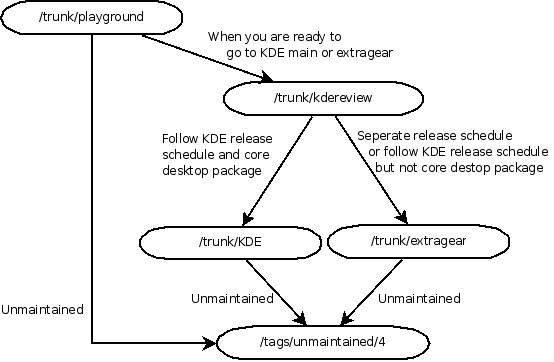
\includegraphics[width=\columnwidth]{images/KDE_application_lifecycle.png}
	\caption{KDE Applicatuion Lifecycle \cite{ApplLife}}
	\label{fig:kde_applLife}
\end{figure}
In Abbildung \ref{fig:kde_applLife} ist schön zu sehen, wie der Lebenszyklus einer KDE-Anwendung aussieht, welche auf Eigeninitiative eines Entwicklers implementiert wurde.\\
Zu Beginn kann lokal mit der KDE-Entwicklungsumgebung programmiert werden. Möchte man seine Anwendung in einem der kommenden Releases enthalten haben, muss man den entsprechenden Code samt Dokumentationspapier ins Subversion Repository committen (Wird momentan komplett auf Git umgestellt). Speziell dafür gibt es die sogenannte Spielwiese (/trunk/playground), auf welcher ohne jede Einschränkung programmiert werden darf.\\
Sollte sich der Entwickler dazu entscheiden, die neue Anwendung gerne zusammen mit dem Release Plan von KDE zu veröffentlichen, wird das Projekt auf die nächste Stufe geschoben, dem sogenannten KDE Review.\\
Dieser Schritt stößt ein zweiwöchiges Review innerhalb der KDE Community an. Führte diese zweiwöchige Phase zu keinerlei Änderungswünschen, hat der Entwickler die Erlaubnis, seine Neuentwicklkung ins produktive KDE zu übernehmen. Je nachdem, ob man dem festen Release Plan von KDE folgen oder darin frei sein möchte, wird das entsprechende Verzeichnis gewählt.\\
Eine letzte Hürde für den KDE Release Plan ist die Zustimmung des entsprechenden Modulkoordinators.\\
Sofern im Review-Status erst noch Änderungen und Bugfixes anstehen, darf je nach Verfügbarkeit des Entwicklers das Projekt bis zur Fehlerbehebung im Review-Status bleiben oder muss auf die Spielwiese zurückgesetzt werden. Dadurch befinden sich nur diejenigen Projekte im Review-Status, an welchen noch regelmäßig weiterentwickelt wird und keine Altlast-Projekte.
\cite{ApplLife}

\subsection{KDE Release Team \cite{KDEReleaseTeam}}
Das KDE Release Team ist zuständig für die Koordination aller offiziellen KDE Releases. Dies beinhaltet unter Anderem die Erstellung eines Zeitplans, die Einplanung von Marketingaufwänden, als auch die Kontrolle zur Einhaltung von Deadlines oder Code-Restriktionen.\\
\begin{figure}[h]
	\centering
	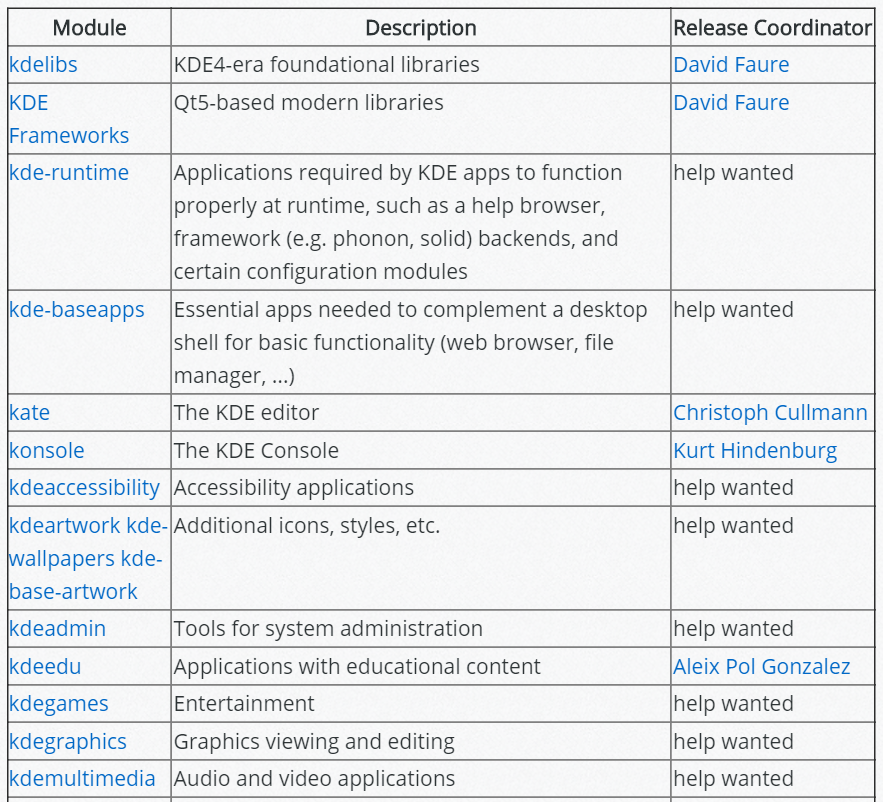
\includegraphics[width=\columnwidth]{images/KDE_module_coordinators.png}
	\caption{Auszug der Liste von KDE-Modulkoordinatoren \cite{KDEReleaseTeam}}
	\label{fig:kde_moduleKoord}
\end{figure}
Der Entscheidungsfindungsprozess soll laut offizieller KDE-Richtlinie öffentlich sein und es können Anregungen sowie Wünsche von allen Seiten eingereicht werden.\\
Personell setzt sich das Release Team aus den einzelnen Modulkoordinatoren der verschiedenen KDE-Module, sowie dem Marketing Team und diversen Personen für die Verwaltung der Planungen zusammen.\\
Die Kommunikation erfolgt wie üblich über Mailing-Listen oder direkte E-Mails. \cite{KDEReleaseTeam} \\ \\
Im Auszug aus Abbildung \ref{fig:kde_moduleKoord} ist deutlich zu sehen, dass nicht einmal die Hälfte der Module bislang einen fixen Modulkoordinator zugewiesen haben. Genau genommen existieren gerade einmal für 9 der 23 KDE-Module solche Personen.\\
Selbst vermeintlich wichtige Posten wie für die Systemadministration sind nicht offiziell besetzt, was sich als großer Schwachpunkt der aktuellen Projekt-Organisation herausstellen könnte.\\ \\
Die Aufgabe des gesamten Release Teams besteht erstens darin, sicherzustellen, dass sich die Neuentwicklungen in einem auslieferbaren Zustand befinden.\\
Die zweite Kernkompetenz liegt darin, neue Features für zukünftige Releases zu sammeln und zu organisieren. Dabei entscheidet das Release Team auch, welche Features wirklich umgesetzt oder verworfen werden. \cite{KDEReleaseTeam} \\ \\
Zusammenfassend lässt sich sagen, dass das Release Team eine zentrale Instanz für die Organisation der Projekte darstellt. Es beherbergt die Überwachung geplanter Entwicklungen, als auch die Entscheidungskraft für künftige Entwicklungen.

\subsection{KDE Release Schedule - Beispiel Plasma 5 \cite{KDEReleaseSchedulePlasma5}}
Dieses Kapitel zeigt einen beispielhaften Release Plan von Plasma 5 (siehe Abbildung \ref{fig:kde_schedulePlasma5}). Der Zeitplan ist das Ergebnis des eben erläuterten Release Teams.\\
Er schlüsselt chronologisch nacheinander die geplanten Versionen zusammen mit dem entsprechenden Release Datum und einer Kurzbeschreibung der enthaltenen Features auf.\\
Ebenso werden die Daten für die entsprechenden Code Freezes vor größeren Releases definiert.
\begin{figure}[h]
	\centering
	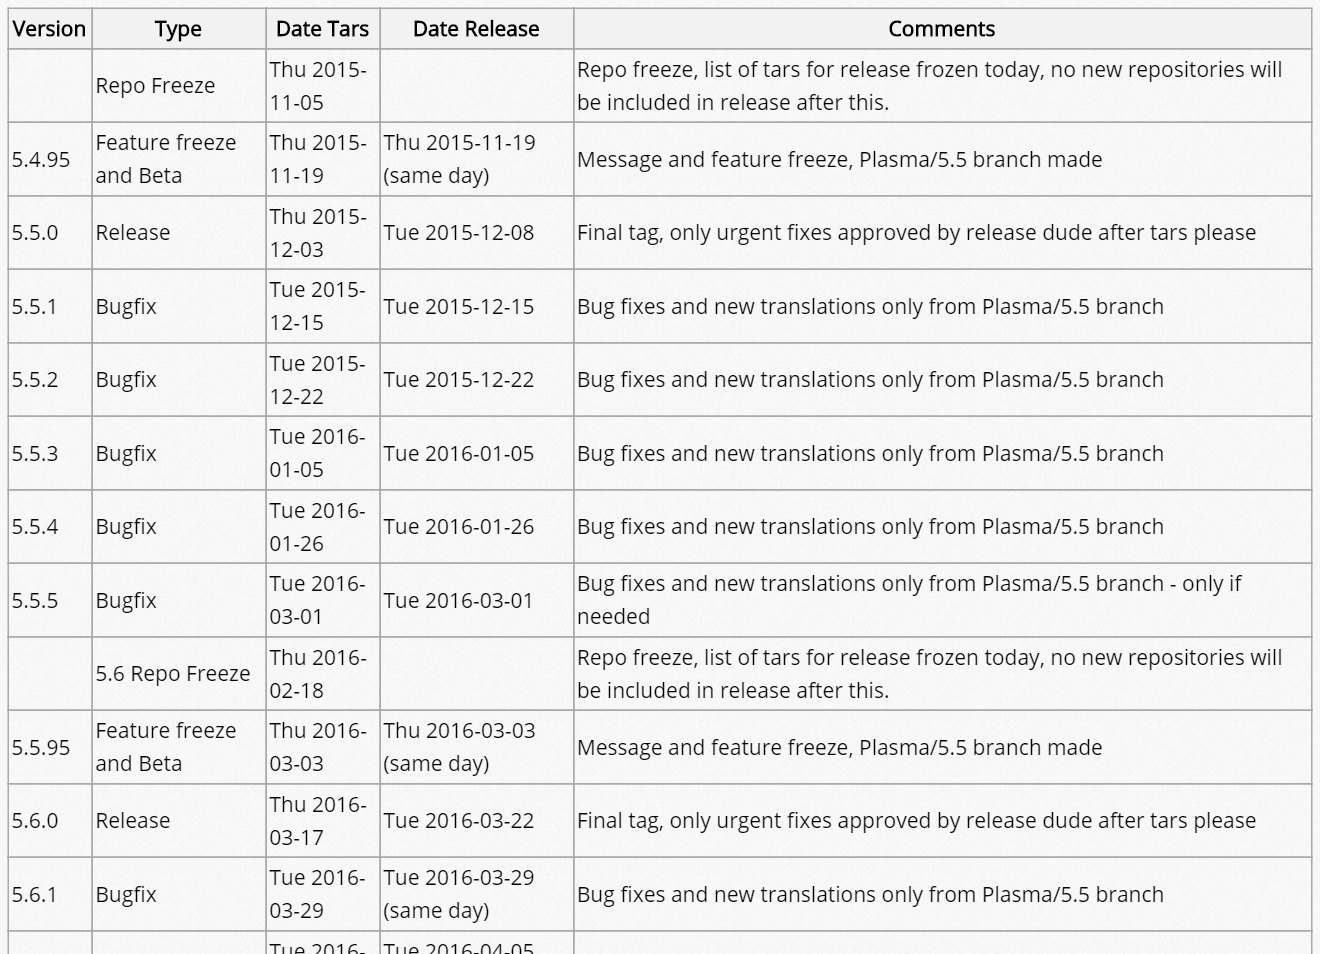
\includegraphics[width=\columnwidth]{images/KDE_schedule_plasma5.png}
	\caption{Auszug des Release Schedule von KDE Plasma 5 \cite{KDEReleaseSchedulePlasma5}}
	\label{fig:kde_schedulePlasma5}
\end{figure}
Der Release Plan orientiert sich an der Planung des Release Teams und in diesem speziellen Fall auch dem Modulkoorinator von Plasma 5. Dieser plant gewöhnlich im Release Team die neuen Features wie in Abbildung \ref{fig:kde_schedulePlasma5}. Alle enthaltenen Features müssen, wie schon erwähnt, zuvor im Release Team abgenommen werden. 
\cite{KDEReleaseSchedulePlasma5}

\subsection{Code Reviews \cite{KDECodeReview}}
Für Code Reviews existieren KDE-seitig diverse Regeln, welche die Codequalität steigern sollen.\\
Thematisch betrachtet decken diese unter Anderem Sicherheitsaspekte, Wartbarkeit, Dokumentation, Stil ab.\\
Wie im KDE Application Lifecycle bereits verdeutlicht, müssen alle Codes im Review-Status, aber auch Bugfixes einem Review unterzogen werden.
\cite{KDECodeReview}

%% Literaturverzeichnis (quellen.bib)
%\bibliography{quellen}{}
%\bibliographystyle{alpha}
%% Abbildungsverzeichnis
%\listoffigures

